\section{Elektronischer Aufbau}

\subsection{Motor}
%Figure
\begin{wrapfigure}{r}{0.65\textwidth}
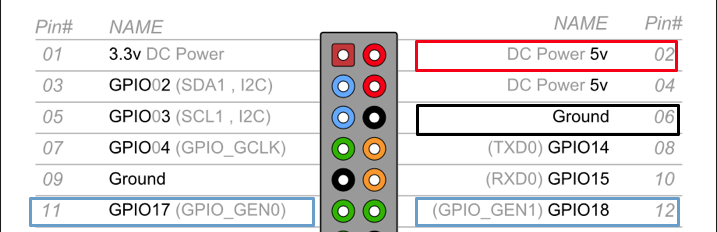
\includegraphics[width=0.9\linewidth]{schaltung/motor-pin}
\caption{GPIO Belegung Motor}
\label{ea:motor-pin}
\end{wrapfigure}
An der Pinbelegung des Motors \ref{eb:motor:tbl} ist zu erkennen, dass der Motor eine Spannung von 9V benöigt. Die Versorgungspanng von 4,3V ist für den eingebauten Controller im Motor. Pin 1 und 2 des Motors müssen mit dem in \ref{eb:pwm} beschriebenen Bauteil verbunden werden (hier Pin 14 und 10 von 754410). Die 9V Motorspannung liegt an Pin 8 (SN754410) an und kommt von einem zusätzlich 9V-Block. Übder die Pins 15 und 11 wird das Bauteil an 2 GPIO's angeschlossen. Weitere benötigte Verbindungen sind die GND, welche alle zusammen verbunden werden und die Versorgungspannung von 4,3V-5V.

Eine Vollständige Belegung der Pins für den Probeaufbau befindet sich in Abbildung \ref{ea:motor-pin}

%Figure
\begin{figure}[h]
  \centering
  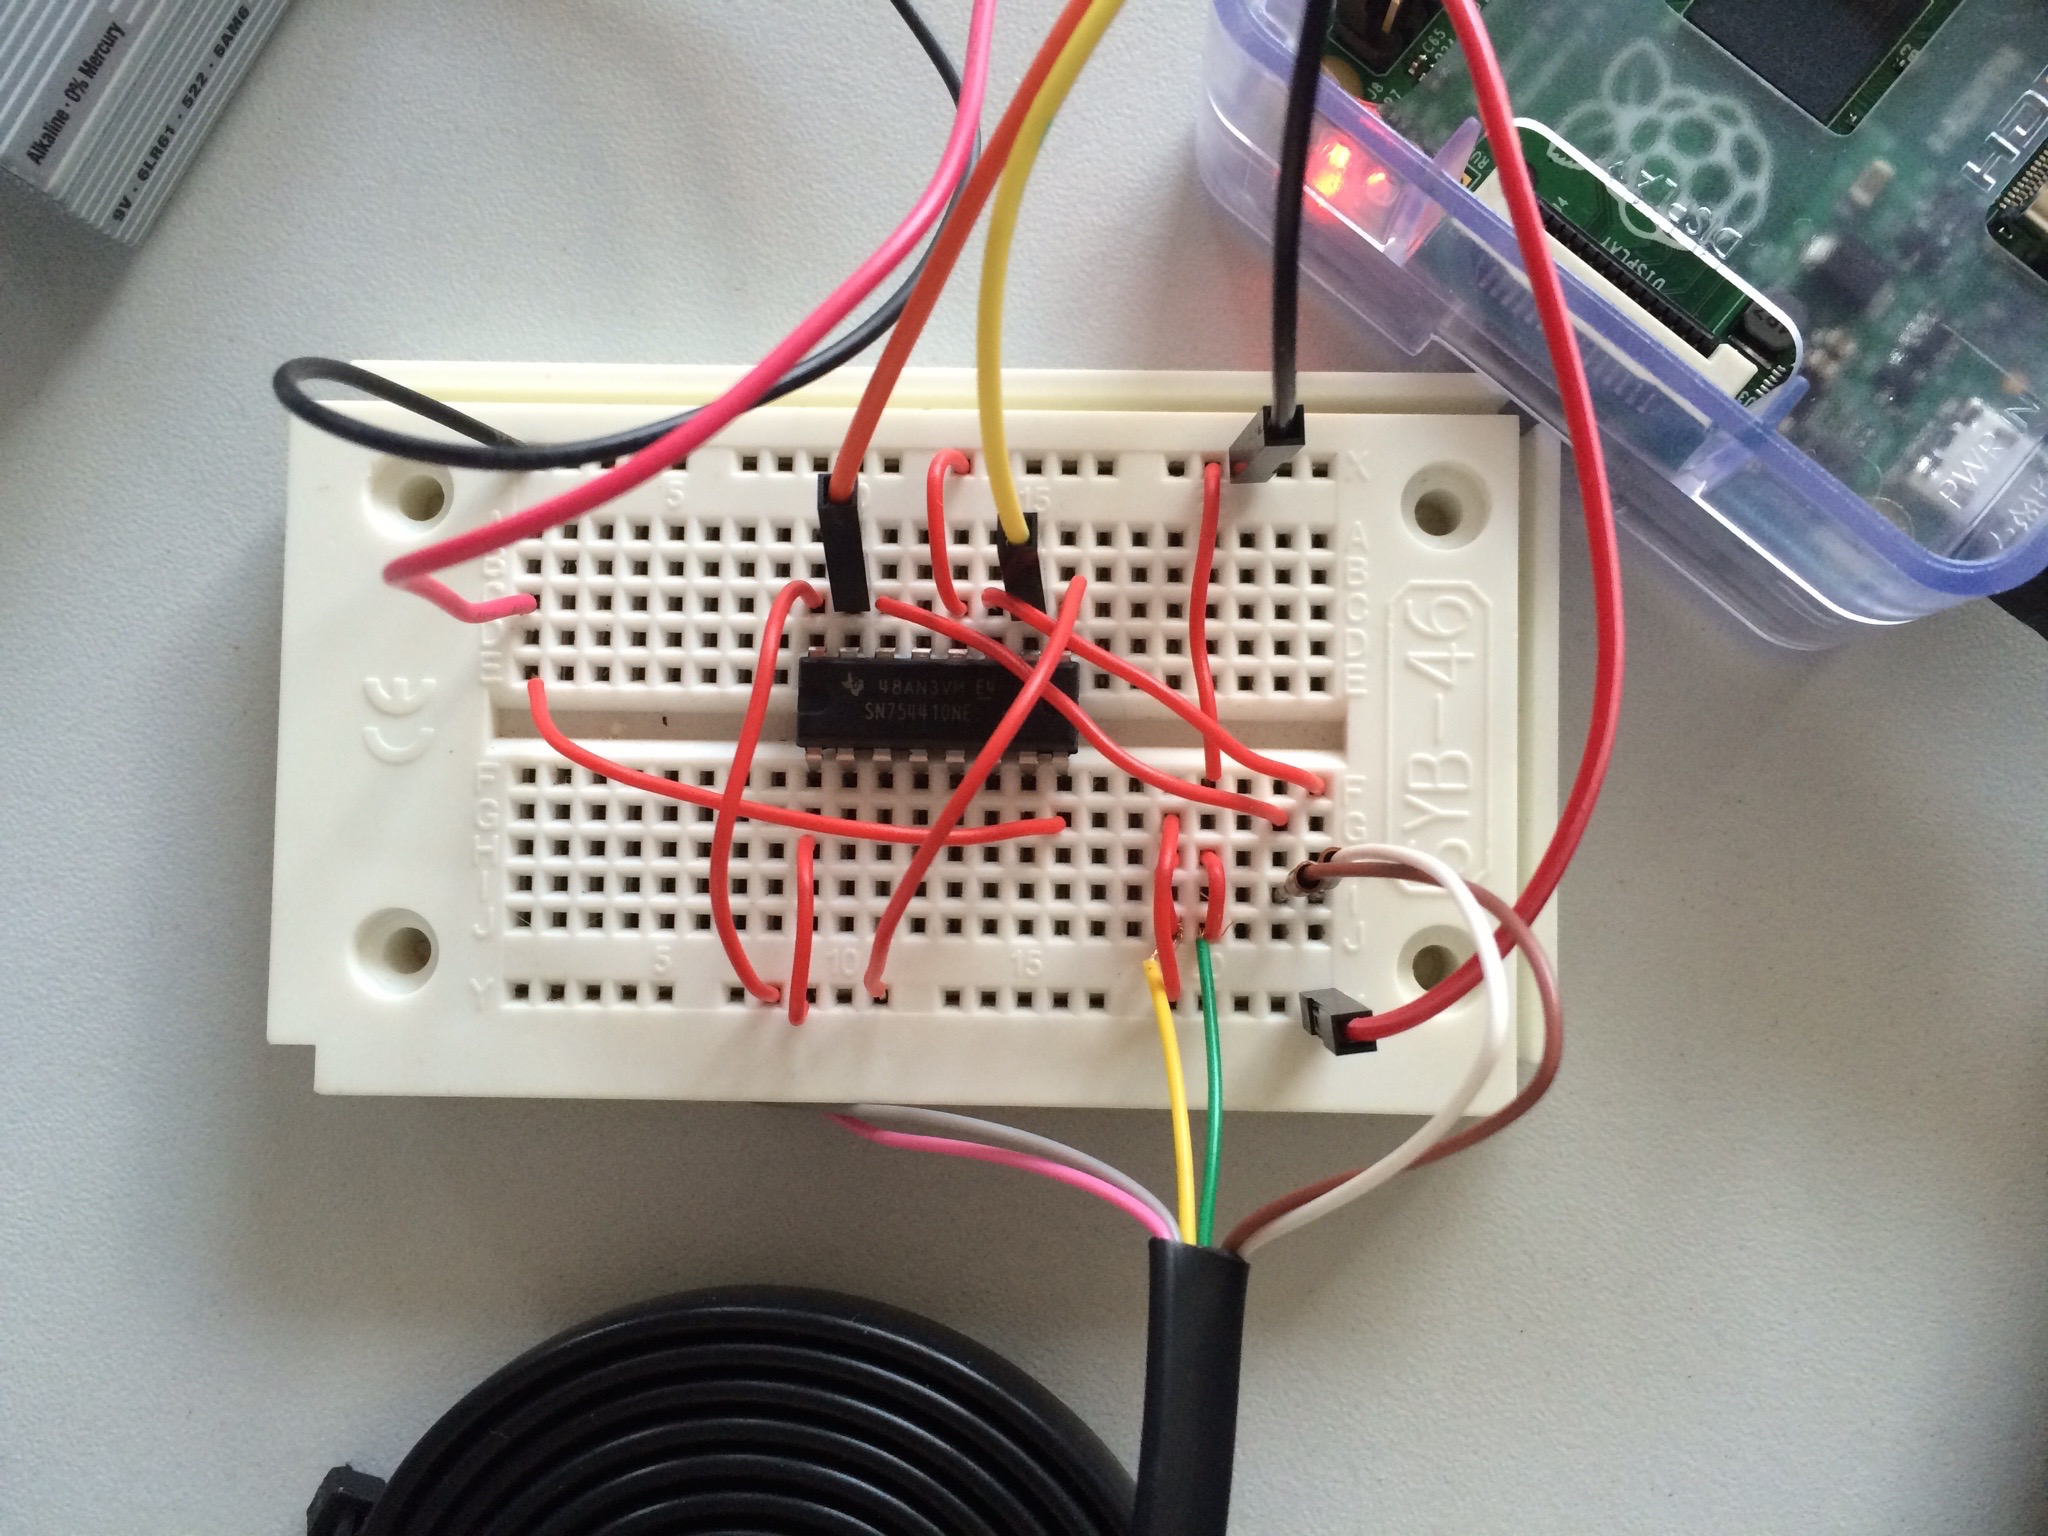
\includegraphics[width=12cm]{schaltung/motor}
  \caption{Probeaufbau Motor}
  \label{schaltung:motor}
\end{figure}

\subsection{Sensor}
%Figure
\begin{wrapfigure}{r}{0.65\textwidth}
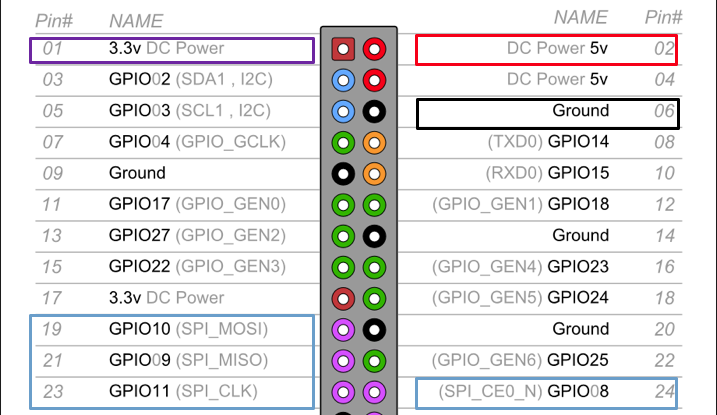
\includegraphics[width=0.9\linewidth]{schaltung/sensor-pin}
\caption{GPIO Belegung Sensor}
\label{ea:sensor-pin}
\end{wrapfigure}

Die Versorgungspannung für den MCP3008 ist hier 3,3V und die Versorgungspannung für die Sensoren sind 4,3V-5V vom Raspberry Pi. Die analogen Sensoren werden an CH0-CH7 an der A/D-Wandler über eine Spannungsteilerschaltung angeschlossen. Der Spannungteiler wird mit einem 10kOhm Widerstand realisiert (in der Probeschaltung 2* 4,7kOhm in Reihe). Mit vier Anschlusskabeln wird der A/D-Wandler über den SPI-Bur am Raspberry Pi angeschlossen. Die Erdung geschieht auch über den Raspberry. Bei dem Spezialfall \emph{Lichtsensor} wird zusätzlich für die Lichtquelle eine Versorgungsspannung benötigt. Da der PIN 5 bei dem \emph{Tastsensor} nicht belegt ist, wird standartmäßig überall der Pin 5 an 4,3V-5V angeschlossen.

%Figure
\begin{figure}[h]
  \centering
  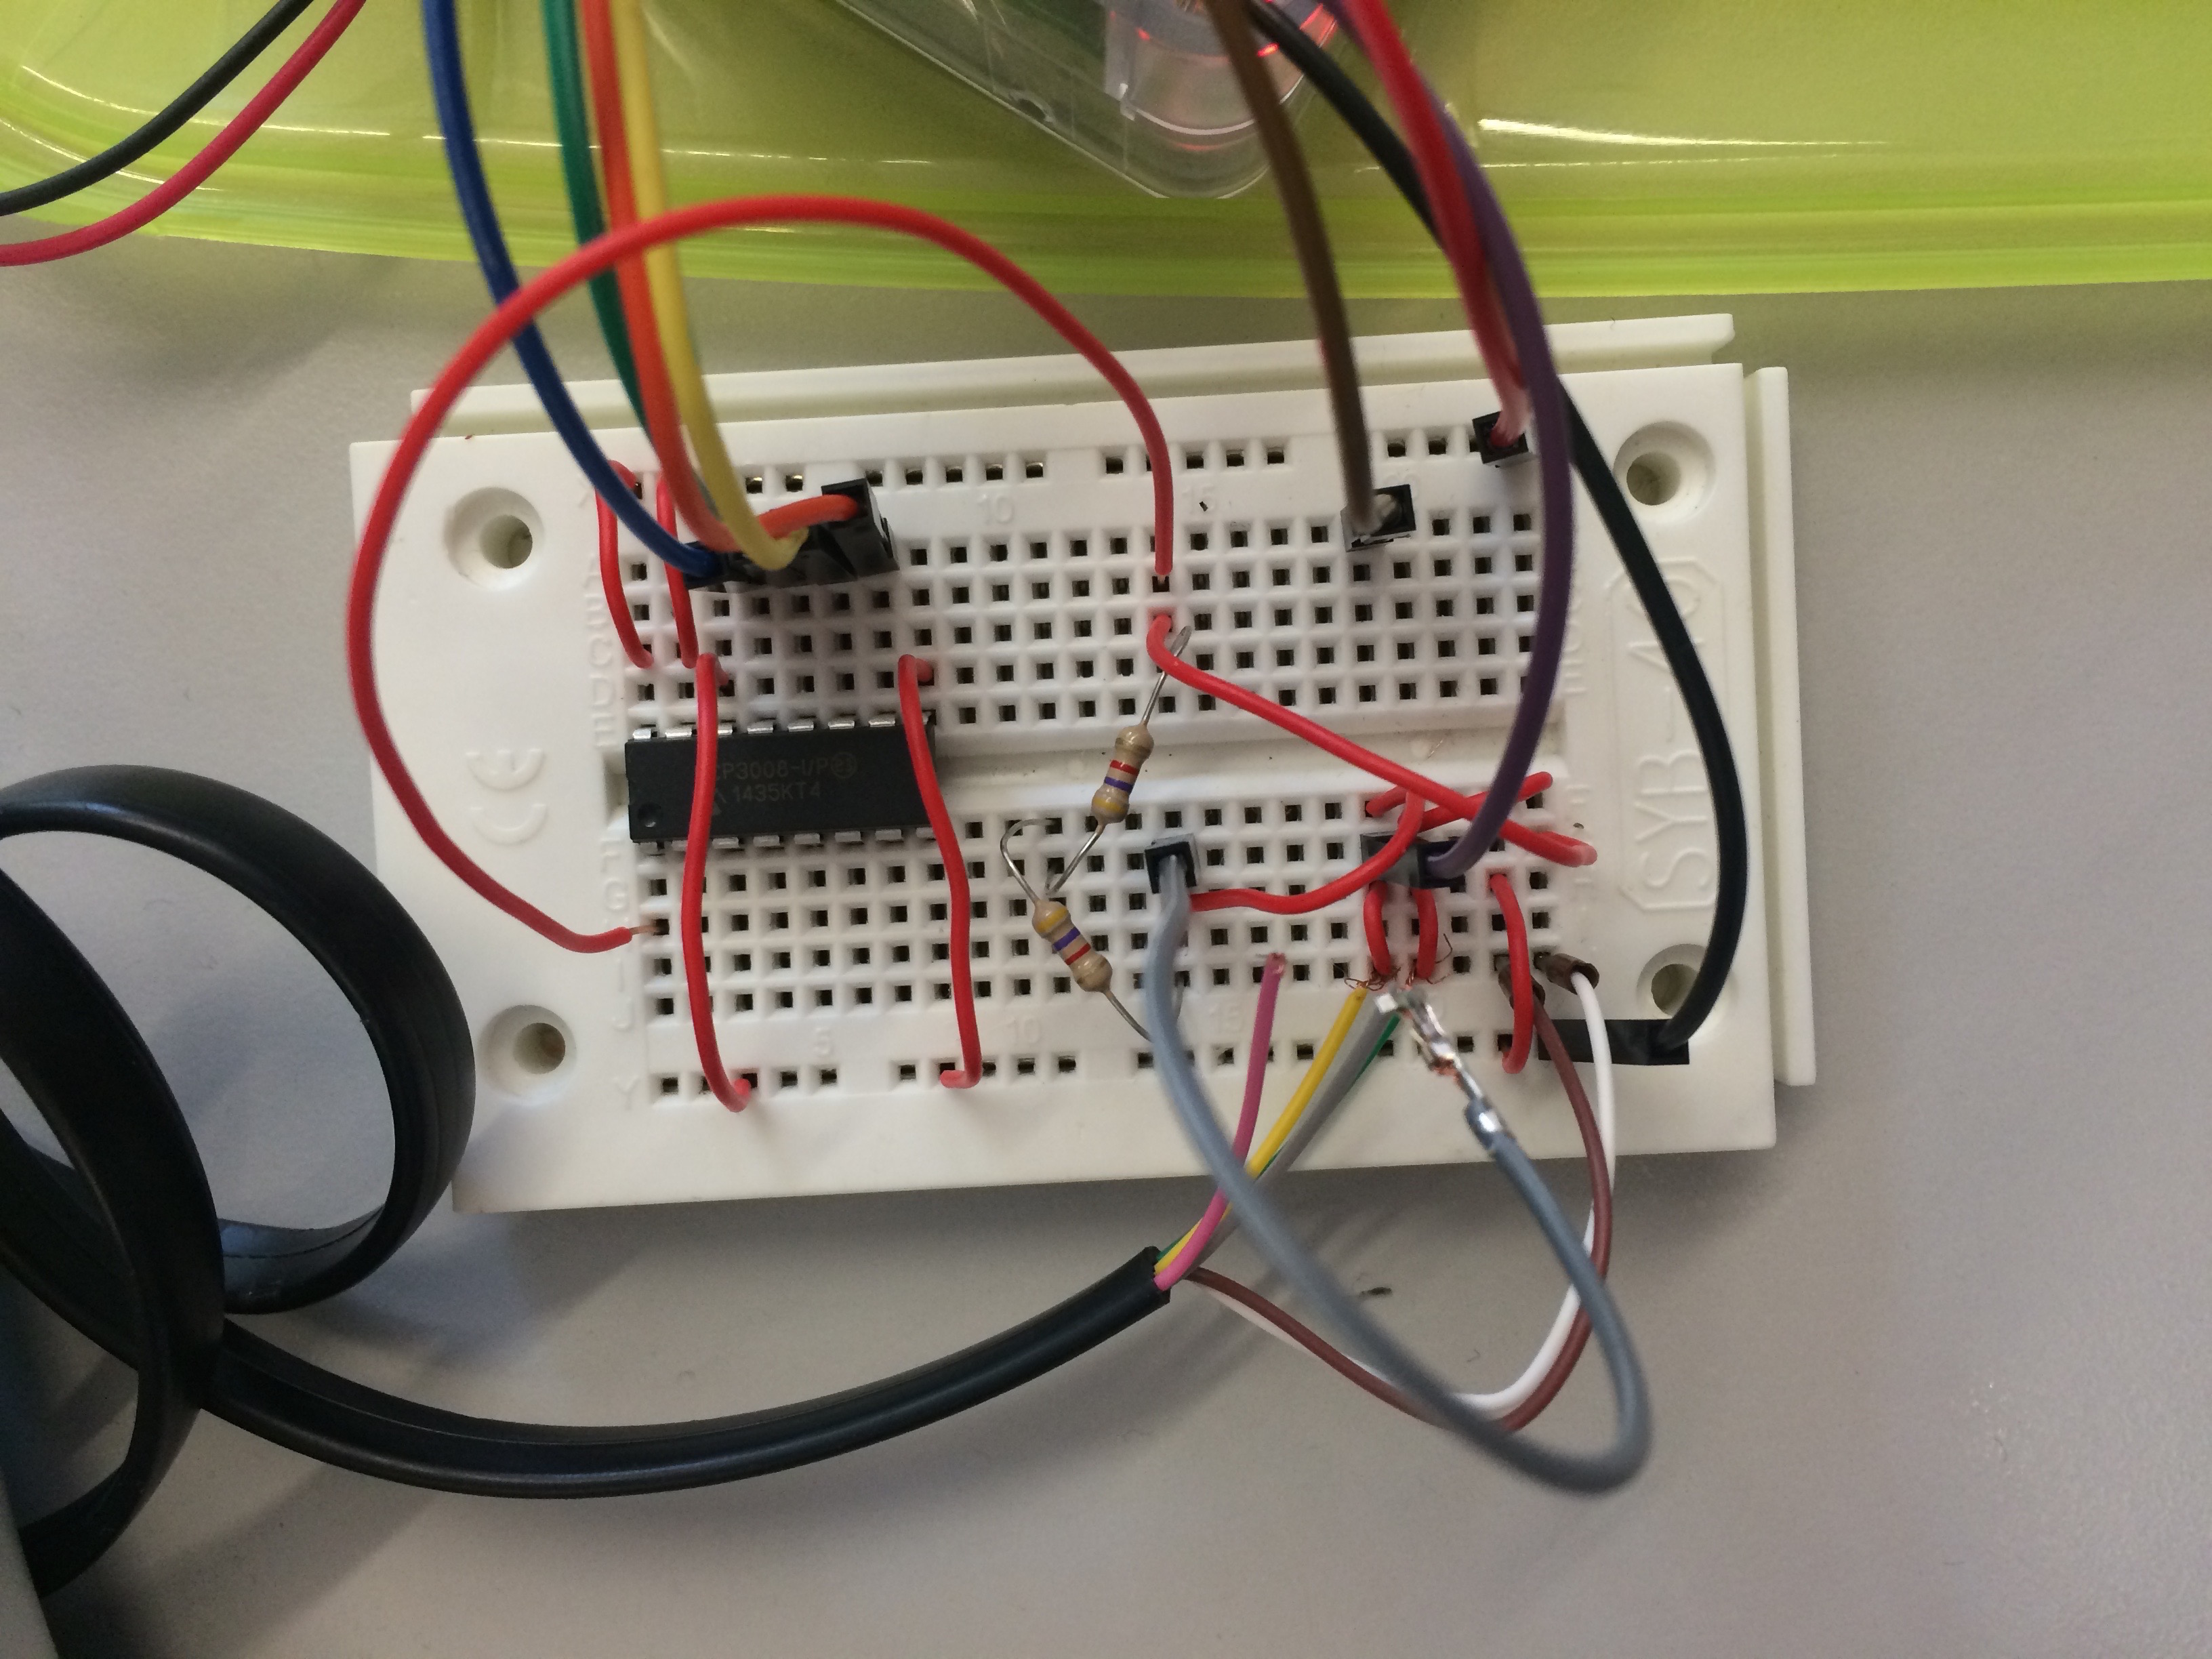
\includegraphics[width=12cm]{schaltung/sensor}
  \caption{Probeaufbau Sensor}
  \label{schaltung:sensor}
\end{figure}

\subsection{Komplett}

Die Herrausforderung die komplette Schaltung zu löten bestand darin die Bauweise so kompakt wir möglich zu gestalten. In der folgenden Liste sind die Bauteile der Schaltung aufgelistet:

\begin{itemize}
  \item 6x female Stecker für NXT Kabel (\EUR{5})
  \item MCP3008 (\EUR{2,5})
  \item SN754410 (\EUR{2,5})
  \item Lochrasterplatine \EUR{1})
  \item 4x 10kOhm Widerstand (\EUR{<1})
  \item 10x female-male Verbindungskabel (<\EUR{1})
  \item Lötzinn und Kupferdraht
\end{itemize}

Die Gesamtkosten der Platine sind mit ca. \EUR{13} sehr gering ausgefallen. Wenn die Kosten eines Raspberry Pi (\EUR{40}) von noch dazugerecht werden, liegen die Gemsamtkosten bei ungefähr \EUR{50}.

Alle Bauelemente lassen sich leicht auf der Lochrasterplatine befestigen. Eine Außnahme stellen die female Stecker da, welche keinen Standartabstand der Pins haben. Hier muss der Kupferdraht direkt angelötet werden.

%Figure
\begin{figure}[h]
  \centering
  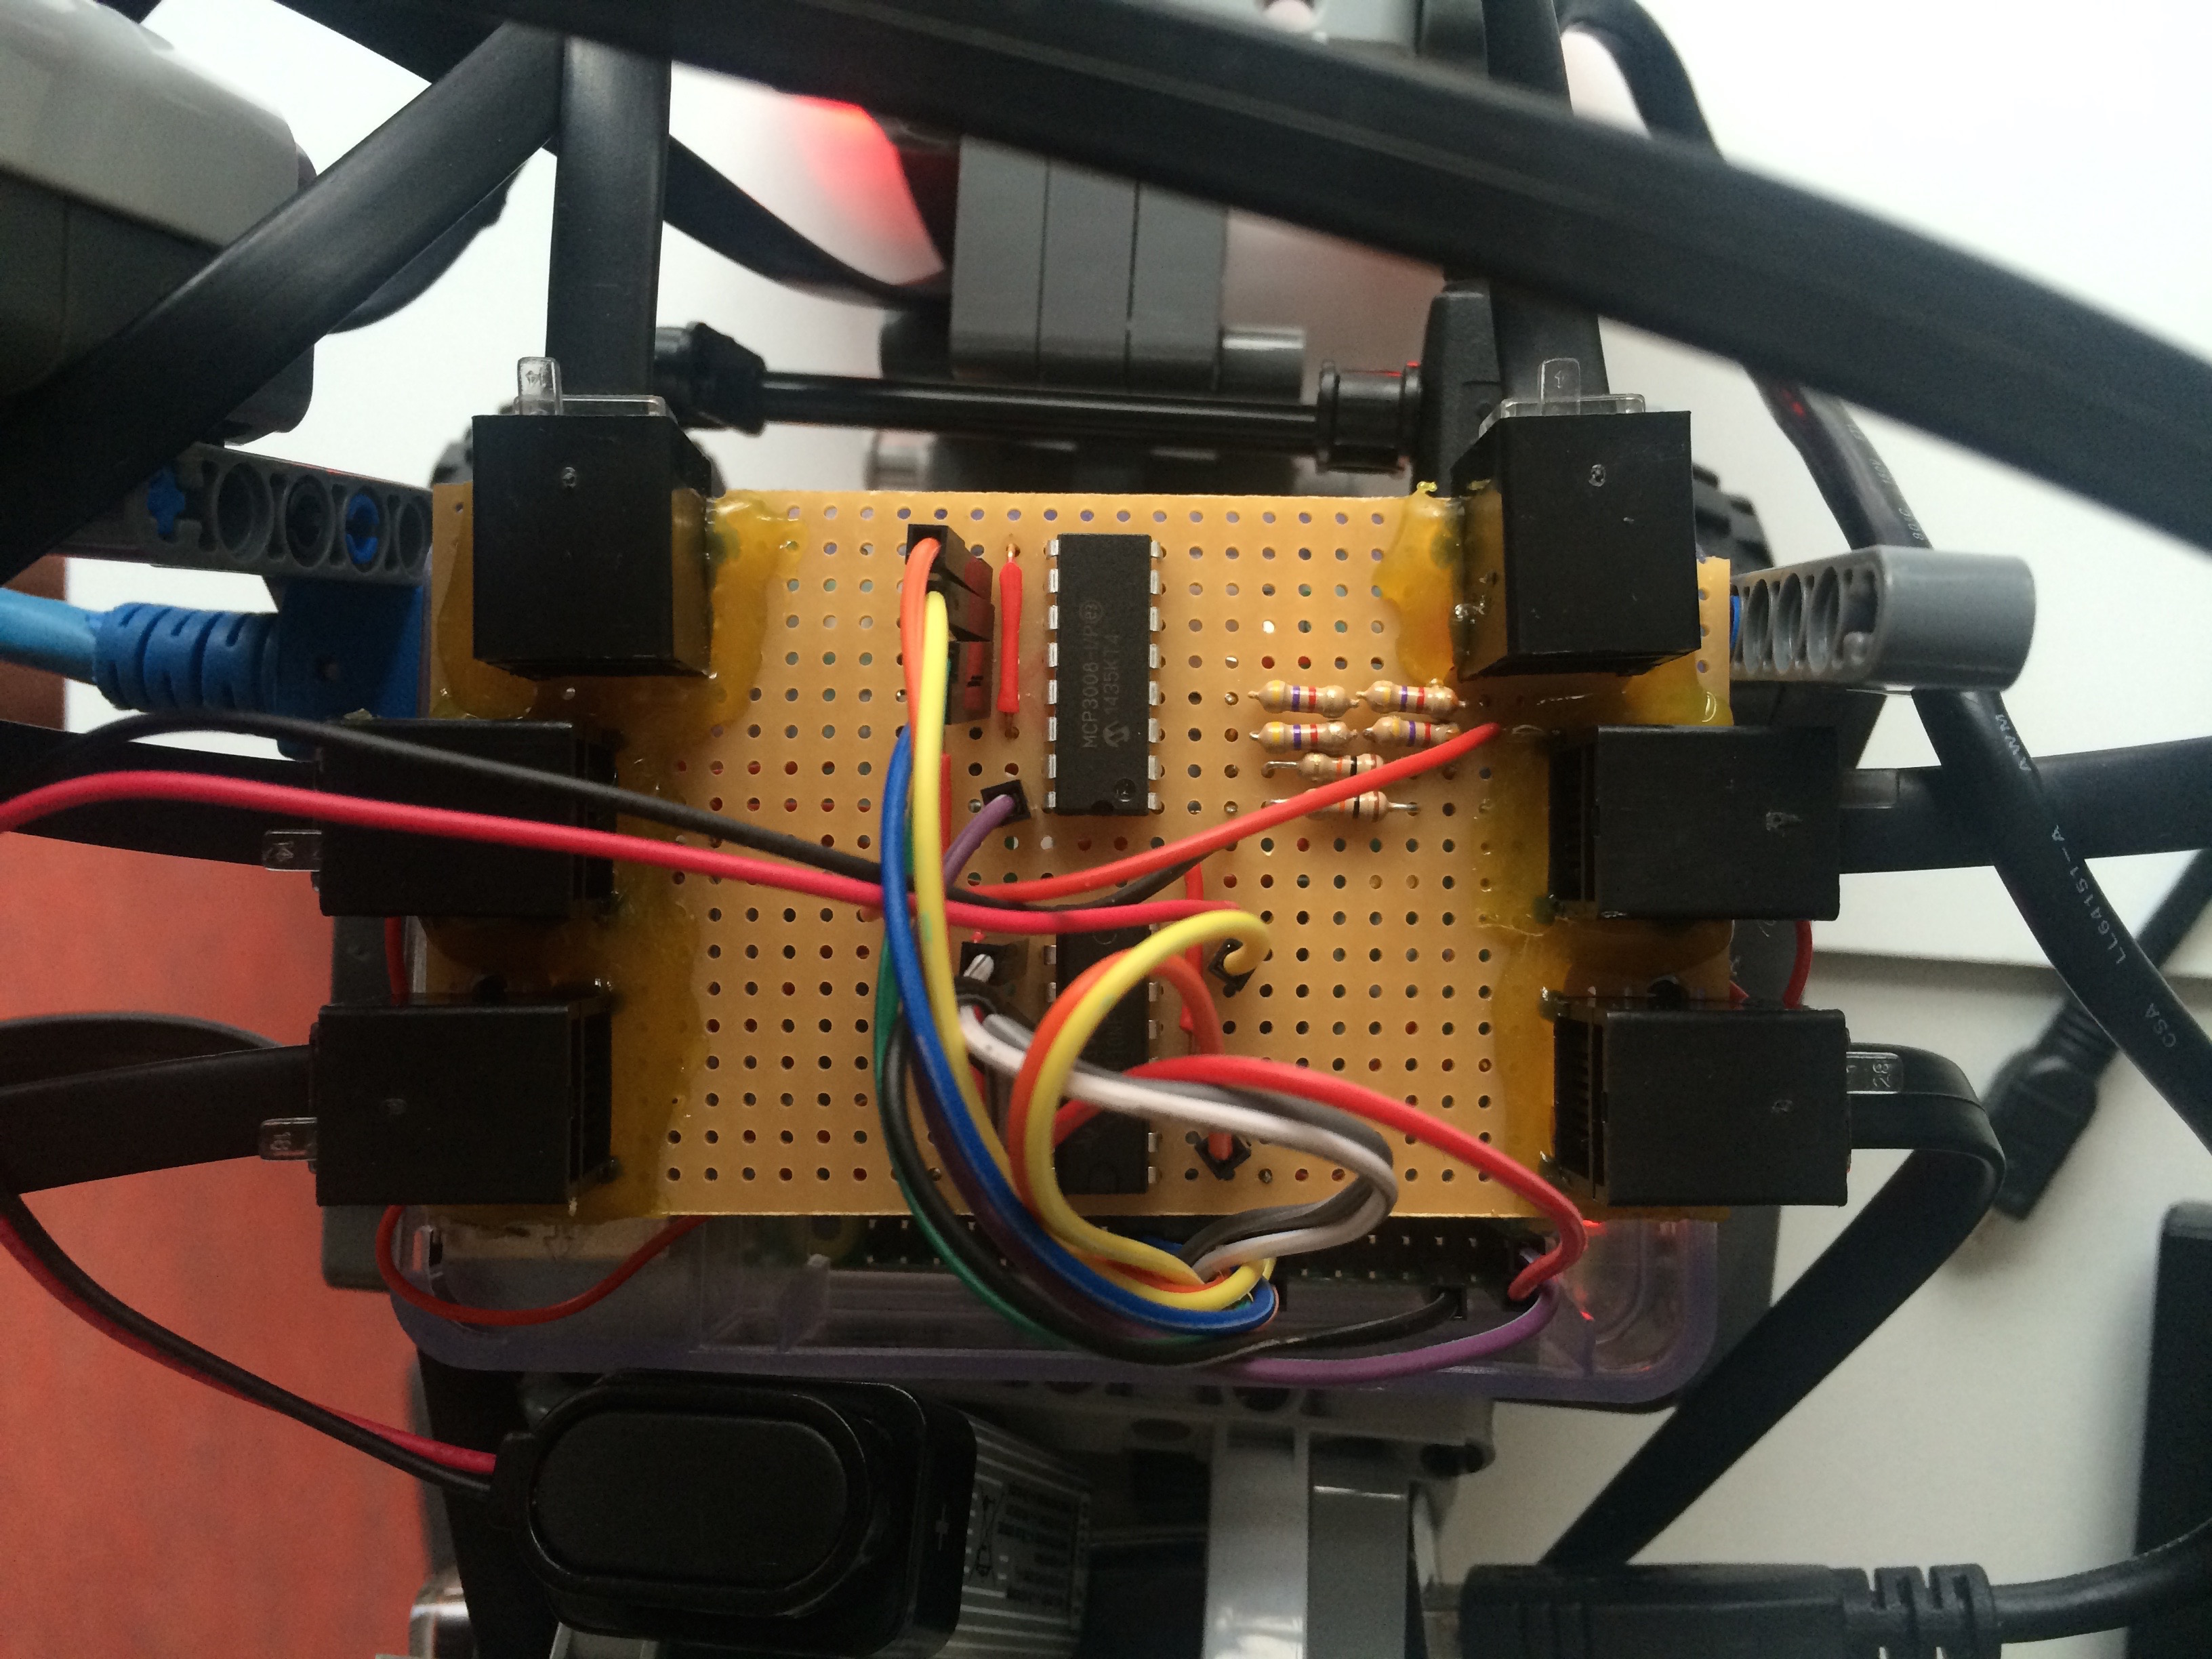
\includegraphics[width=12cm]{schaltung/komplett}
  \caption{Komplette Schaltung}
  \label{schaltung:komplett}
\end{figure}
